\chapter{Implementacija i korisničko sučelje}
		
		
		\section{Korištene tehnologije i alati}
		
			
			Svi članovi tima su sudjelovali u odabiru tehnologija i alata koji će se koristiti za izradu aplikacije. Kao sredstvo komunikacije, odabrana je aplikacija 
			\underbar{WhatsApp}\footnote{\url{https://www.whatsapp.com/}}. Pomoću WhatsApp-a, članovi tima su mogli komunicirati u stvarnom vremenu, razmjenjivati datoteke,
			te se dogovarati o terminima sastanaka. Za izradu UML dijagrama korišten je alat \underbar{Astah Professional}\footnote{\url{http://astah.net/editions/professional}}
			dok se \underbar{Git}\footnote{\url{https://git-scm.com/}} koristio kao sustav za upravljanje izvornim kodom. Na web platformi \underbar{GitHub}\footnote{\url{https://github.com/}} je dostupan udaljeni repozitorij projekta.
			Za izradu dokumentacije korišten je \underbar{LaTeX}\footnote{\url{https://www.latex-project.org/}}.
			Za razvojno okruženje korišten je \underbar{Visual Studio Code}\footnote{\url{https://code.visualstudio.com/}} budući da je vrlo popularan za razvoj web i mobilnih aplikacija kao i drugih programa te je vrlo pregledan i jednostavan za korištenje.
			Za izradu naše web aplikacije korišteni su biblioteka \underbar{React}\footnote{\url{https://reactjs.org/}} i jezik \underbar{Javascript}\footnote{\url{https://www.javascript.com/}} za izradu frontenda.
			React je biblioteka za izradu korisničkih sučelja koja je održavana od strane Facebooka. 
			React se koristi za izradu jednostraničnih aplikacija (engl. single-page application) ili mobilnih aplikacija.
			React se fokusira na izradu korisničkog sučelja, dok se za ostale funkcionalnosti aplikacije koristi JavaScript - dinamički tipizirani programski jezik koji je jedan od najpopularnijih na svijetu za izradu web aplikacija.
			Za izradu backenda korišten je jezik \underbar{Python}\footnote{\url{https://www.python.org/}} i biblioteka \underbar{Django}\footnote{\url{https://www.djangoproject.com/}}.
			Django, web framework za Python, poslužio je za razvoj backend dijela aplikacije, dok se za ostale funkcionalnosti koristi Python - još jedan dinamički tipizirani programski jezik često korišten za izradu web aplikacija.

			
			\eject 
		
	
		\section{Ispitivanje programskog rješenja}
			

			\subsection{Ispitivanje komponenti}
\begin{lstlisting}[breaklines=true]
class ViewTest(TestCase):
	def setUp(self):
		Group.objects.create(name='Zaposlenici')
		Group.objects.create(name='Direktori')

		self.base_url = "/api/"
		self.zaposlenik = User.objects.create_user(username='test', password='test')
		Group.objects.get(name='Zaposlenici').user_set.add(self.zaposlenik)
		self.direktor = User.objects.create_user(username='test2', password='test2')
		Group.objects.get(name='Direktori').user_set.add(self.direktor)

		self.client = Client()
		self.zaposlenik_token = self.client.post(self.base_url + 'token/', {'username': 'test', 'password': 'test'}).data.get('access')
		self.direktor_token = self.client.post(self.base_url + 'token/', {'username': 'test2', 'password': 'test2'}).data.get('access')

		self.interni_dokument1 = InterniDokument.objects.create(tekstDokumenta='tekst 1', linkSlike='link 1', vrijemeSkeniranja=timezone.datetime(2021, 5, 5, 10, 10, 10, tzinfo=pytz.UTC), korisnik=self.direktor)
		self.interni_dokument2 = InterniDokument.objects.create(tekstDokumenta='tekst 2', linkSlike='link 2', vrijemeSkeniranja=timezone.datetime(2021, 5, 5, 10, 10, 10, tzinfo=pytz.UTC), korisnik=self.zaposlenik)


	# Testovi funckionalnosti korisnika

	def test_promijeni_lozinku(self):
		self.assertTrue(self.zaposlenik.check_password('test'))

		response = self.client.put(
			self.base_url + 'promijeniLozinku/',
			{"trenutnaLozinka": "test", "novaLozinka": "test"},
			HTTP_AUTHORIZATION='Bearer ' + self.zaposlenik_token,
			content_type='application/json'
		)
		self.assertEquals(response.status_code, 418)

		response = self.client.put(
			self.base_url + 'promijeniLozinku/',
			{"trenutnaLozinka": "test", "novaLozinka": "new_password"},
			HTTP_AUTHORIZATION='Bearer ' + self.zaposlenik_token,
			content_type='application/json'
		)
		self.assertEquals(response.status_code, 200)
		self.zaposlenik.refresh_from_db()
		self.assertFalse(self.zaposlenik.check_password('test'))
		self.assertTrue(self.zaposlenik.check_password('new_password'))

	def test_dodaj_korisnika(self):
		response = self.client.post(
			self.base_url + 'dodajKorisnika/',
			{"username": "test3", "password": "test3"},
			HTTP_AUTHORIZATION='Bearer ' + self.zaposlenik_token,
			content_type='application/json'
		)
		self.assertEquals(response.status_code, 403)

		response = self.client.post(
			self.base_url + 'dodajKorisnika/',
			{"username": "test3", "password": "test3", "email": "abc@example.com", "ime": "test", "prezime": "test", "group": "Zaposlenici"},
			HTTP_AUTHORIZATION='Bearer ' + self.direktor_token,
			content_type='application/json'
		)
		self.assertEquals(response.status_code, 201)
		self.assertTrue(User.objects.filter(username="test3").exists())
		user = User.objects.get(username="test3")
		self.assertTrue(Group.objects.get(name='Zaposlenici').user_set.filter(username="test3").exists())
		self.assertTrue(user.check_password('test3'))
		self.assertEquals(user.email, "abc@example.com")
		self.assertEquals(user.first_name, "test")
		self.assertEquals(user.last_name, "test")
		
	def test_dohvati_korisnike_grupe(self):
		response = self.client.get(
			self.base_url + 'dohvatiKorisnikeGrupe/Zaposlenici',
			HTTP_AUTHORIZATION='Bearer ' + self.zaposlenik_token,
			content_type='application/json'
		)
		
		self.assertEqual(response.status_code, 200)
		data = response.json()
		self.assertEqual(data['korisnici'], [{'id': self.zaposlenik.id, 'username': 'test'}])
		
		response = self.client.get(
			self.base_url + 'dohvatiKorisnikeGrupe/Direktori',
			HTTP_AUTHORIZATION='Bearer ' + self.direktor_token,
			content_type='application/json'
		)
		
		self.assertEqual(response.status_code, 200)
		data = response.json()
		self.assertEqual(data['korisnici'], [{'id': self.direktor.id, 'username': 'test2'}])
		
	def test_dohvati_specijalizirane_racunovodje(self):
		Group.objects.create(name='Računovođe')
		računovođa = User.objects.create_user(username='test3', password='test3')
		Group.objects.get(name='Računovođe').user_set.add(računovođa)

		SpecijalizacijaRačunovođe.objects.create(korisnik=računovođa, tipSpecijalizacije=0)
		
		response = self.client.get(
			self.base_url + 'dohvatiSpecijaliziraneRačunovođe/abc',
			HTTP_AUTHORIZATION='Bearer ' + self.zaposlenik_token,
			content_type='application/json'
		)
		self.assertEqual(response.status_code, 400)
		
		response = self.client.get(
			self.base_url + 'dohvatiSpecijaliziraneRačunovođe/Računi',
			HTTP_AUTHORIZATION='Bearer ' + self.zaposlenik_token,
			content_type='application/json'
		)
		
		self.assertEqual(response.status_code, 200)
		data = response.json()
		self.assertEqual(data['korisnici'], [{'id': računovođa.id, 'username': 'test3'}])
		
		response = self.client.get(
			self.base_url + 'dohvatiSpecijaliziraneRačunovođe/Ponude',
			HTTP_AUTHORIZATION='Bearer ' + self.zaposlenik_token,
			content_type='application/json'
		)
		
		self.assertEqual(response.status_code, 200)
		data = response.json()
		self.assertEqual(data['korisnici'], [])
		
		
	# Testovi funkcionalnosti rada s dokumentima
	
	def test_moji_dokumenti(self):
		response = self.client.get(
			self.base_url + 'mojiDokumenti/',
			HTTP_AUTHORIZATION='Bearer ' + self.direktor_token,
			content_type='application/json'
		)
		self.assertEqual(response.status_code, 200)
		data = response.json()
		self.assertEqual(len(data['dokumenti']), 1)
		self.assertEqual(data['dokumenti'][0]['id'], self.interni_dokument1.id)
		
	def test_svi_dokumenti(self):
		response = self.client.get(
			self.base_url + 'sviDokumenti/',
			HTTP_AUTHORIZATION='Bearer ' + self.direktor_token,
			content_type='application/json'
		)
		self.assertEqual(response.status_code, 200)
		data = response.json()
		self.assertEqual(len(data['dokumenti']), 2)
		self.assertEqual(data['dokumenti'][0]['id'], self.interni_dokument1.id)
		self.assertEqual(data['dokumenti'][1]['id'], self.interni_dokument2.id)

	def test_označi_točnost_skeniranja(self):
		self.assertFalse(self.interni_dokument2.točnoSkeniran)
		response = self.client.put(
			self.base_url + 'označiTočnostSkeniranja/' + str(self.interni_dokument2.id),
			{"tocnost": True},
			HTTP_AUTHORIZATION='Bearer ' + self.zaposlenik_token,
			content_type='application/json'
		)
		self.assertEqual(response.status_code, 200)
		self.interni_dokument2.refresh_from_db()
		self.assertTrue(self.interni_dokument2.točnoSkeniran)
		
	def test_potpiši(self):
		self.assertFalse(self.interni_dokument1.potpisaoDirektor)
		response = self.client.put(
			self.base_url + 'potpiši/' + str(self.interni_dokument1.id),
			HTTP_AUTHORIZATION='Bearer ' + self.direktor_token,
			content_type='application/json'
		)
		
		self.assertEqual(response.status_code, 200)
		self.interni_dokument1.refresh_from_db()
		self.assertTrue(self.interni_dokument1.potpisaoDirektor)
		
	def test_dodijeli_revizora(self):
		revizori = Group.objects.create(name='Revizori')
		revizor = User.objects.create_user(username='test3', password='test3')
		revizori.user_set.add(revizor)
		
		self.assertIsNone(self.interni_dokument1.revizor)
		response = self.client.put(
			self.base_url + 'dodijeliRevizora/' + str(self.interni_dokument1.id),
			{"korisnik_id": revizor.id},
			HTTP_AUTHORIZATION='Bearer ' + self.zaposlenik_token,
			content_type='application/json'
		)
		
		self.assertEqual(response.status_code, 200)
		self.interni_dokument1.refresh_from_db()
		self.assertEqual(self.interni_dokument1.revizor, revizor)
		
		response = self.client.put(
			self.base_url + 'dodijeliRevizora/' + str(self.interni_dokument1.id),
			{"korisnik_id": self.direktor.id},
			HTTP_AUTHORIZATION='Bearer ' + self.zaposlenik_token,
			content_type='application/json'
		)
		self.assertEqual(response.status_code, 400)
		
		response = self.client.put(
			self.base_url + 'dodijeliRevizora/' + '0',
			{"korisnik_id": revizor.id},
			HTTP_AUTHORIZATION='Bearer ' + self.zaposlenik_token,
			content_type='application/json'
		)
		self.assertEqual(response.status_code, 404)
		
	def test_arhiviraj(self):
		Group.objects.create(name='Računovođe')
		računovođa = User.objects.create_user(username='test3', password='test3')
		Group.objects.get(name='Računovođe').user_set.add(računovođa)
		
		računovođa_token = self.client.post(self.base_url + 'token/', {'username': 'test3', 'password': 'test3'}).data.get('access')
		
		pk = self.interni_dokument1.pk
		tekst = self.interni_dokument1.tekstDokumenta
		self.assertTrue(InterniDokument.objects.filter(pk=pk).exists())
		self.assertFalse(InterniDokumentArhiviran.objects.filter(dokumentId=pk).exists())
		response = self.client.put(
			self.base_url + 'arhiviraj/' + str(self.interni_dokument1.id),
			HTTP_AUTHORIZATION='Bearer ' + računovođa_token,
			content_type='application/json'
		)

		self.assertEqual(response.status_code, 200)
		self.assertFalse(InterniDokument.objects.filter(pk=pk).exists())
		
		documents = InterniDokumentArhiviran.objects.filter(dokumentId=pk)
		self.assertTrue(documents.exists())
		self.assertTrue(len(documents) == 1)
		self.assertTrue(documents[0].tekstDokumenta == tekst)
		
		
Rezultat izvođenja u vscodeu:
Found 10 test(s).
Creating test database for alias 'default'...
System check identified no issues (0 silenced).
..........
----------------------------------------------------------------------
Ran 10 tests in 11.969s

OK
Destroying test database for alias 'default'...
\end{lstlisting}
			
			
			\subsection{Ispitivanje sustava}
			
			Test 1 (test\_login\_fail):\\
			Otvorimo URI web stranice. Pokušamo se ulogirati s neispravnom kombinacijom korisničkog imena i zaporke.
			Osiguramo da se pojavi alert s tekstom "Pogrešno korisničko ime ili lozinka".\\
			\\
			Test 2 (test\_login\_and\_logout):\\
			Otvorimo URI web stranice. Ulogiramo se s ispravnim korisničkim imenom i lozinkom. Izlogiramo se.
			Osiguramo da smo opet završili na login stranici.\\
			\\
			Test 3 (test\_change\_password):\\
			Otvorimo URI web stranice. Ulogiramo se s ispravnim korisničkim imenom i lozinkom. Pokušamo promijeniti
			lozinku korisnika pri čemu unesemo pogrešnu trenutnu lozinku. Osiguramo da se pojavi alert teksta
			"Unesite ispravnu trenutnu lozinku" i da se lozinka korisnika nije promijenila. Ponovimo isto ali s
			ispravnom trenutnom lozinkom i novom lozinkom istom kao i starom. Osiguramo da se pojavi alert teksta
			"Nova lozinka mora biti različita od stare" i da se lozinka korisnika nije promijenila. Ponovimo isto s
			ispravnom trenutnom lozinkom i novom lozinkom različitom od stare. Osiguramo da se pojavio alert teksta
			"Lozinka uspješno promijenjena" i da lozinka korisnika promijenila. Vratimo lozinku na staru.\\
			\\
			Test 4 (test\_add\_new\_employee):\\
			Otvorimo URI web stranice. Ulogiramo se s ispravnim direktorovim korisničkim imenom i lozinkom.
			Otvorimo stranicu za dodavanje novog zaposlenika. Pokušamo dodati novog zaposlenika s istim korisničkim
			imena kao neki već postojeći. Osiguramo da se pojavi alert teksta "Greška prilikom dodavanja zaposlenika".
			Ponovimo isto ali s ispravim korisničkim imenom. Osiguramo da se pojavi alert teksta "Zaposlenik uspješno
			dodan". Osiguramo da se novi korisnik pojavio u bazi sa svim potrebnim atributima. Izbrišemo novonastalog
			korisnika.
			
			\eject 
		
		
		\section{Dijagram razmještaja}
			
			\begin{figure}[H]
				Dijagram razmještaja na slici 5.1 prikazuje topologiju sklopovlja i programsku potporu web-aplikacije. Sustav je baziran na arhitekturi
				"klijent-poslužitelj". Komunikacija između računala korisnika i frontend poslužiteljskog računala, kao i između frontend i backend poslužiteljskog
				računala, odvija se preko HTTP veze. Korisnici pristupaju web-aplikaciji koristeći web preglednik te im frontend poslužiteljsko računalo, na kojem
				se nalazi frontend web poslužitelj, daje odgovarajući prikaz. Na backend poslužiteljskom računalu nalazi se Docker u kojemu se nalaze backend web
				poslužitelj i Tesseract, a Postgres baza nalazi se na poslužiteljskom računalu baze podataka koje je povezano s backend poslužiteljskim računalom.
				\newline
				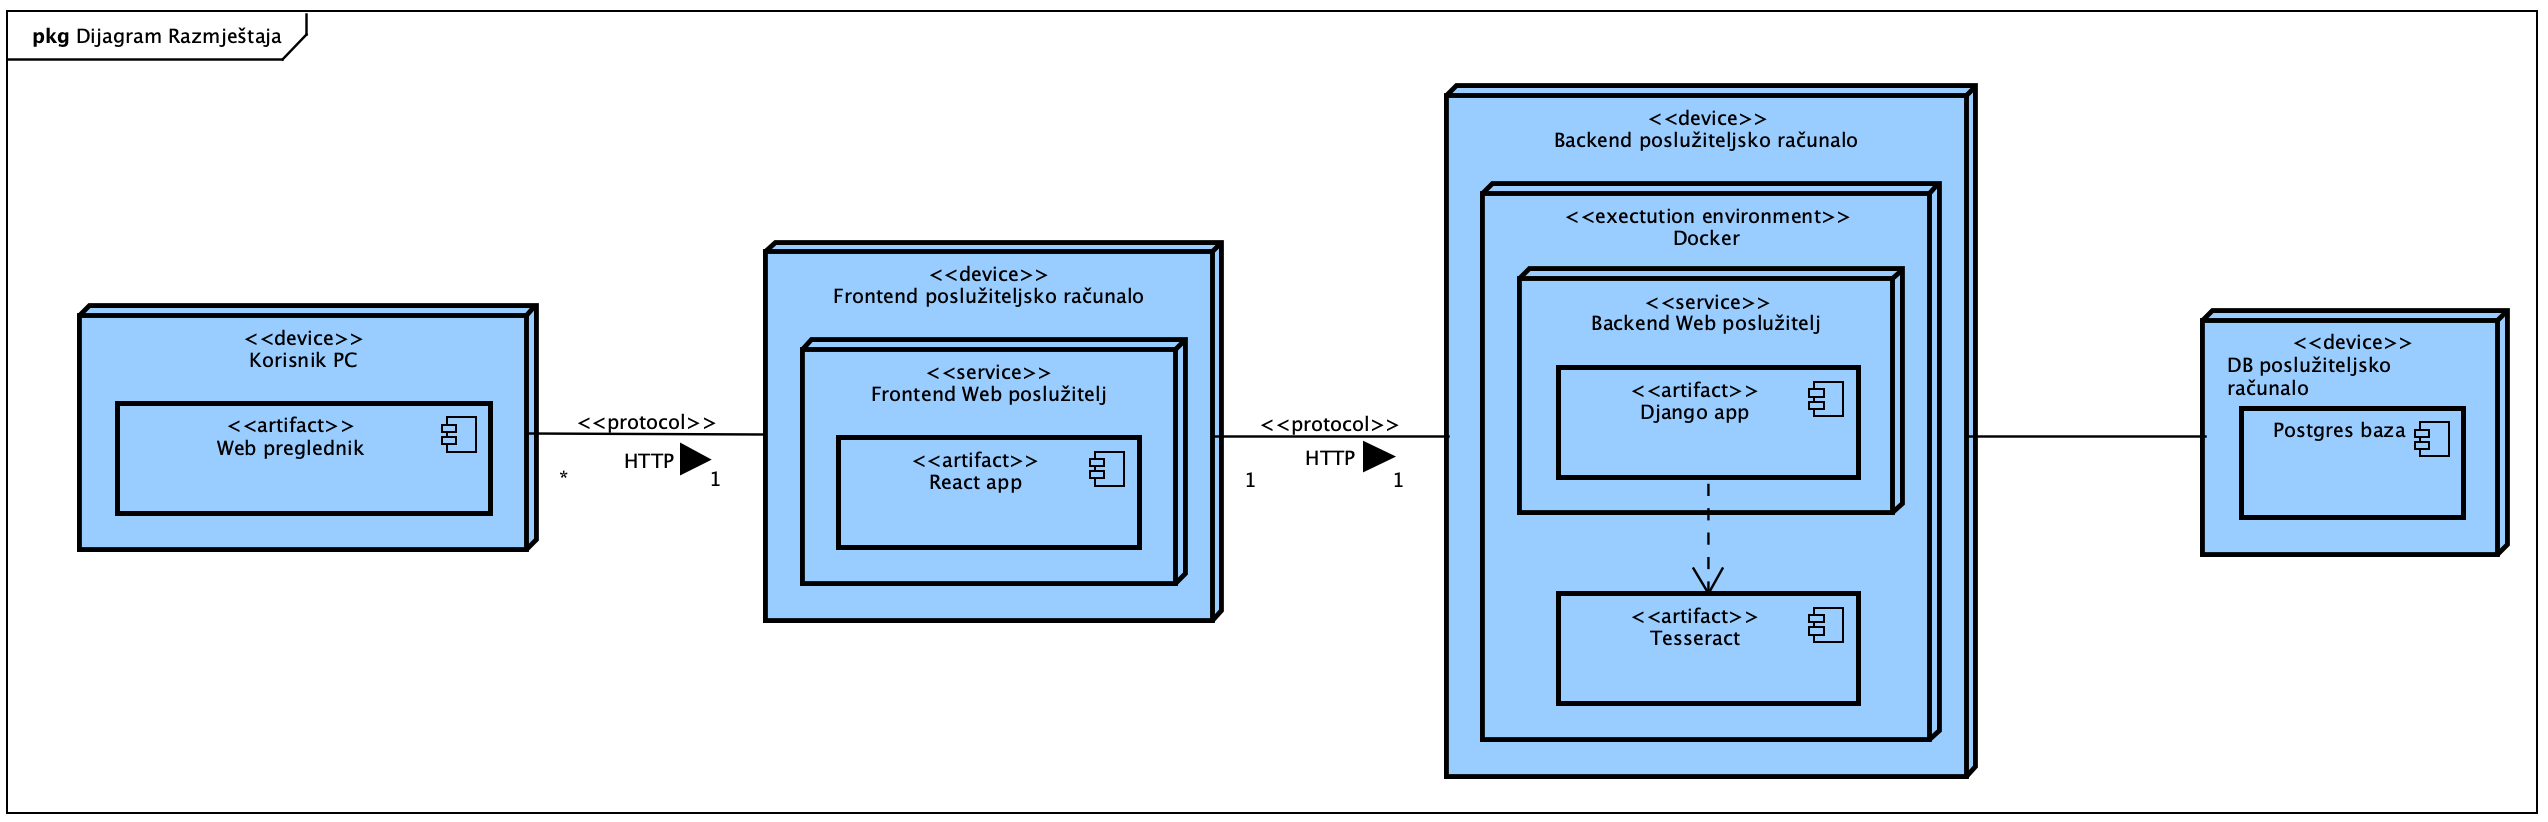
\includegraphics[width=\textwidth]{slike/Deployment.png}
				\caption{Dijagram razmještaja}
				\label{fig:Deployment}
			\end{figure}
			\eject 
		
		\section{Upute za puštanje u pogon}
		
			\textbf{\textit{dio 2. revizije}}\\
		
			 \textit{U ovom poglavlju potrebno je dati upute za puštanje u pogon (engl. deployment) ostvarene aplikacije. Na primjer, za web aplikacije, opisati postupak kojim se od izvornog kôda dolazi do potpuno postavljene baze podataka i poslužitelja koji odgovara na upite korisnika. Za mobilnu aplikaciju, postupak kojim se aplikacija izgradi, te postavi na neku od trgovina. Za stolnu (engl. desktop) aplikaciju, postupak kojim se aplikacija instalira na računalo. Ukoliko mobilne i stolne aplikacije komuniciraju s poslužiteljem i/ili bazom podataka, opisati i postupak njihovog postavljanja. Pri izradi uputa preporučuje se \textbf{naglasiti korake instalacije uporabom natuknica} te koristiti što je više moguće \textbf{slike ekrana} (engl. screenshots) kako bi upute bile jasne i jednostavne za slijediti.}
			
			
			 \textit{Dovršenu aplikaciju potrebno je pokrenuti na javno dostupnom poslužitelju. Studentima se preporuča korištenje neke od sljedećih besplatnih usluga: \href{https://aws.amazon.com/}{Amazon AWS}, \href{https://azure.microsoft.com/en-us/}{Microsoft Azure} ili \href{https://www.heroku.com/}{Heroku}. Mobilne aplikacije trebaju biti objavljene na F-Droid, Google Play ili Amazon App trgovini.}
			
			
			\eject 